\let\negmedspace\undefined
\let\negthickspace\undefined
\documentclass[journal]{IEEEtran}
\usepackage[a5paper, margin=10mm, onecolumn]{geometry}
%\usepackage{lmodern} % Ensure lmodern is loaded for pdflatex
\usepackage{tfrupee} % Include tfrupee package

\setlength{\headheight}{1cm} % Set the height of the header box
\setlength{\headsep}{0mm}     % Set the distance between the header box and the top of the text

\usepackage{gvv-book}
\usepackage{gvv}
\usepackage{cite}
\usepackage{amsmath,amssymb,amsfonts,amsthm}
\usepackage{algorithmic}
\usepackage{graphicx}
\usepackage{textcomp}
\usepackage{xcolor}
\usepackage{txfonts}
\usepackage{listings}
\usepackage{enumitem}
\usepackage{mathtools}
\usepackage{gensymb}
\usepackage{comment}
\usepackage[breaklinks=true]{hyperref}
\usepackage{tkz-euclide} 
\usepackage{listings}
% \usepackage{gvv}                                        
\def\inputGnumericTable{}                                 
\usepackage[latin1]{inputenc}                                
\usepackage{color}                                            
\usepackage{array}                                            
\usepackage{longtable}                                       
\usepackage{calc}                                             
\usepackage{multirow} 
\usepackage{hhline}                                           
\usepackage{ifthen}                                           
\usepackage{lscape}
\usepackage{circuitikz}
\tikzstyle{block} = [rectangle, draw, fill=blue!20, 
    text width=4em, text centered, rounded corners, minimum height=3em]
\tikzstyle{sum} = [draw, fill=blue!10, circle, minimum size=1cm, node distance=1.5cm]
\tikzstyle{input} = [coordinate]
\tikzstyle{output} = [coordinate]

\begin{document}
\bibliographystyle{IEEEtran}
\vspace{3cm}

\title{MatGeo Assignment 1.2.13}
\author{AI25BTECH11007}
 \maketitle
% \newpage
% \bigskip
{\let\newpage\relax\maketitle}

\renewcommand{\thefigure}{\theenumi}
\renewcommand{\thetable}{\theenumi}
\setlength{\intextsep}{10pt} % Space between text and floats


\numberwithin{equation}{enumi}
\numberwithin{figure}{enumi}
\renewcommand{\thetable}{\theenumi}
\noindent
\textbf{Question:}\\
If (1, 2), (4, y), (x, 6) and (3, 5) are the vertices of a parallelogram taken in order, find
x and y.\\
\noindent
\textbf{Solution:}\\
Let us solve the given equation theoretically and then verify the solution computationally \\
According to the question, \\

We are given the vertices of a parallelogram in order:

\text{Given the vertices of a parallelogram: } 
$$A(1,2), \; B(4,y), \; C(x,6), \; D(3,5).$$

\text{Property: In a parallelogram, diagonals bisect each other.}

\text{So, midpoint of } AC = \text{midpoint of } BD.

\begin{equation}
\frac{1}{2}
\myvec{
1 + x \\
2 + 6
}
=
\frac{1}{2}
\myvec{
4 + 3 \\
y + 5
}
\end{equation}

\begin{equation}
\myvec{
\frac{1+x}{2} \\
\frac{8}{2}
}
=
\myvec{
\frac{7}{2} \\
\frac{y+5}{2}
}
\end{equation}

\begin{equation}
\frac{1+x}{2} = \frac{7}{2}, 
\quad 
\frac{8}{2} = \frac{y+5}{2}
\end{equation}

\begin{equation}
x = 6, 
\quad 
y = 3
\end{equation}

\begin{equation}
\therefore \; x=6, \; y=3
\end{equation}

\begin{figure}[H]
   
    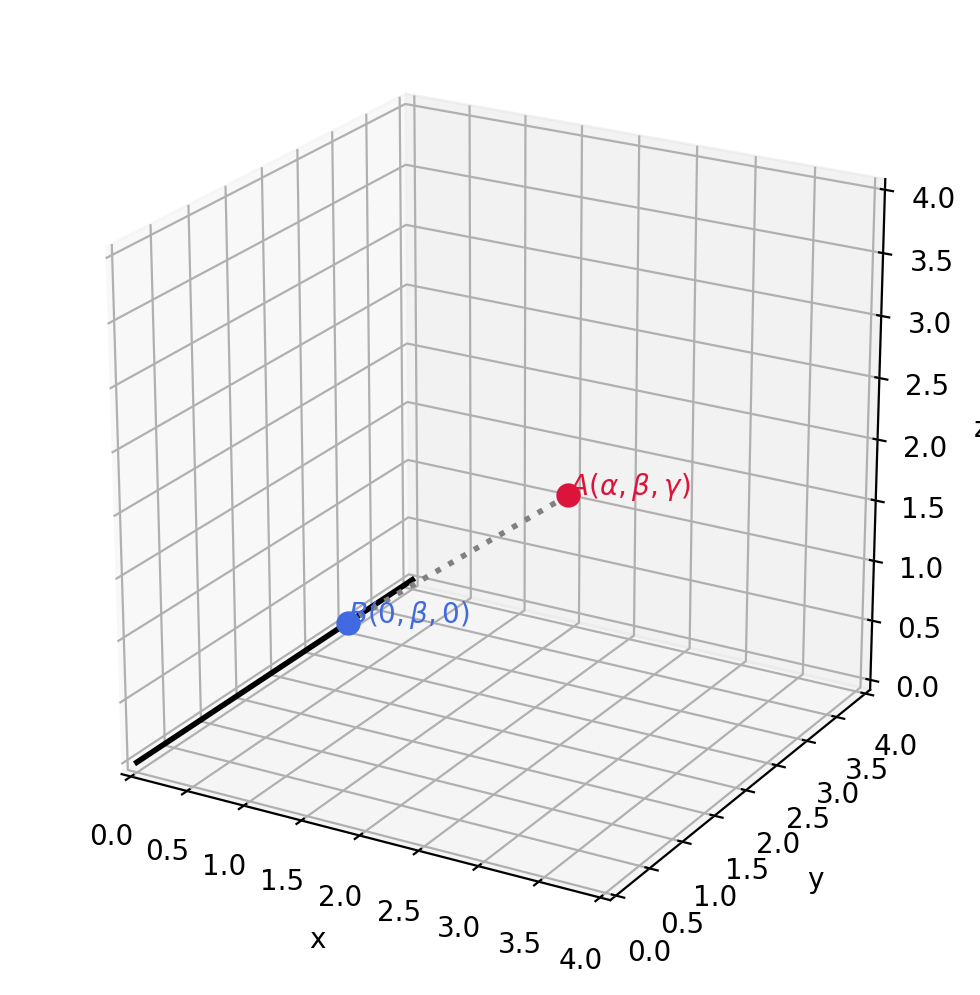
\includegraphics[width=0.75\linewidth]{figs/fig1.png}
\caption{The visual of the parallelogram with vertices labeled and diagonals shown}
    \label{fig:figs/fig1.png}
\end{figure}
\noindent
From the figure it is clearly verified that theoritical solution matches with the computational solution.

\end{document}
